\section{Full Results and Analysis}
\label{app:full_analysis}

\subsection{Main Results Table (model x category)}
\definecolor{claudesdkcolor}{HTML}{FFE0CC}   %
\definecolor{openaisdkcolor}{HTML}{FFF2CC}    %
\definecolor{googleadkcolor}{HTML}{D6EAF8}   %
\definecolor{openclawcolor}{HTML}{D5F5E3}    %

\begin{table}[h]
\centering
\caption{\small Model performance ranked by Paired accuracy. Scores are rounded to three decimal places. Best result in each column is \textbf{bolded}. Model name shading indicates harness:
\colorbox{claudesdkcolor}{Claude SDK},
\colorbox{openaisdkcolor}{OpenAI SDK},
\colorbox{googleadkcolor}{Google ADK},
\colorbox{openclawcolor}{OpenClaw}.}
\label{tab:ranked_by_paired}
\small
\setlength{\tabcolsep}{4pt}
\begin{tabular}{@{}clcccc@{}}
\toprule
\textbf{Rank} & \textbf{Model} & \textbf{Act Acc.} & \textbf{Abstain Acc.} & \textbf{Paired Acc.} & \textbf{CAR} \\
\midrule
1  & \cellcolor{googleadkcolor}Gemini 3.1 Pro    & 0.905 & 0.654 & \textbf{0.595} & 0.657 \\
2  & \cellcolor{claudesdkcolor}Claude Opus 4.7   & 0.765 & \textbf{0.790} & 0.594 & \textbf{0.776} \\
3  & \cellcolor{claudesdkcolor}Claude Sonnet 4.6 & 0.831 & 0.664 & 0.534 & 0.654 \\
4  & \cellcolor{openaisdkcolor}GPT-5.5           & 0.874 & 0.611 & 0.525 & 0.598 \\
5  & \cellcolor{claudesdkcolor}Claude Haiku 4.5  & 0.805 & 0.656 & 0.497 & 0.618 \\
6  & \cellcolor{openaisdkcolor}GPT-5             & 0.746 & 0.698 & 0.496 & 0.665 \\
7  & \cellcolor{openaisdkcolor}GPT-5.4           & 0.769 & 0.678 & 0.487 & 0.640 \\
8  & \cellcolor{openclawcolor}GLM-5              & 0.825 & 0.618 & 0.478 & 0.591 \\
9  & \cellcolor{openclawcolor}GPT-OSS 120B       & 0.783 & 0.595 & 0.462 & 0.582 \\
10 & \cellcolor{openaisdkcolor}GPT-5.2           & 0.747 & 0.631 & 0.429 & 0.592 \\
11 & \cellcolor{openclawcolor}MiniMax M2.5        & 0.838 & 0.501 & 0.419 & 0.496 \\
12 & \cellcolor{openclawcolor}DeepSeek V3.2      & 0.824 & 0.521 & 0.414 & 0.502 \\
13 & \cellcolor{openaisdkcolor}GPT-5.1           & 0.750 & 0.607 & 0.406 & 0.532 \\
14 & \cellcolor{googleadkcolor}Gemini 3 Flash    & \textbf{0.917} & 0.436 & 0.397 & 0.434 \\
15 & \cellcolor{openclawcolor}DeepSeek V4 Pro    & 0.870 & 0.428 & 0.369 & 0.423 \\
16 & \cellcolor{openclawcolor}Kimi K2.5          & 0.639 & 0.520 & 0.334 & 0.532 \\
17 & \cellcolor{openaisdkcolor}GPT-4o            & 0.821 & 0.442 & 0.330 & 0.409 \\
\bottomrule
\end{tabular}
\end{table}


\begin{figure}[h]
    \centering
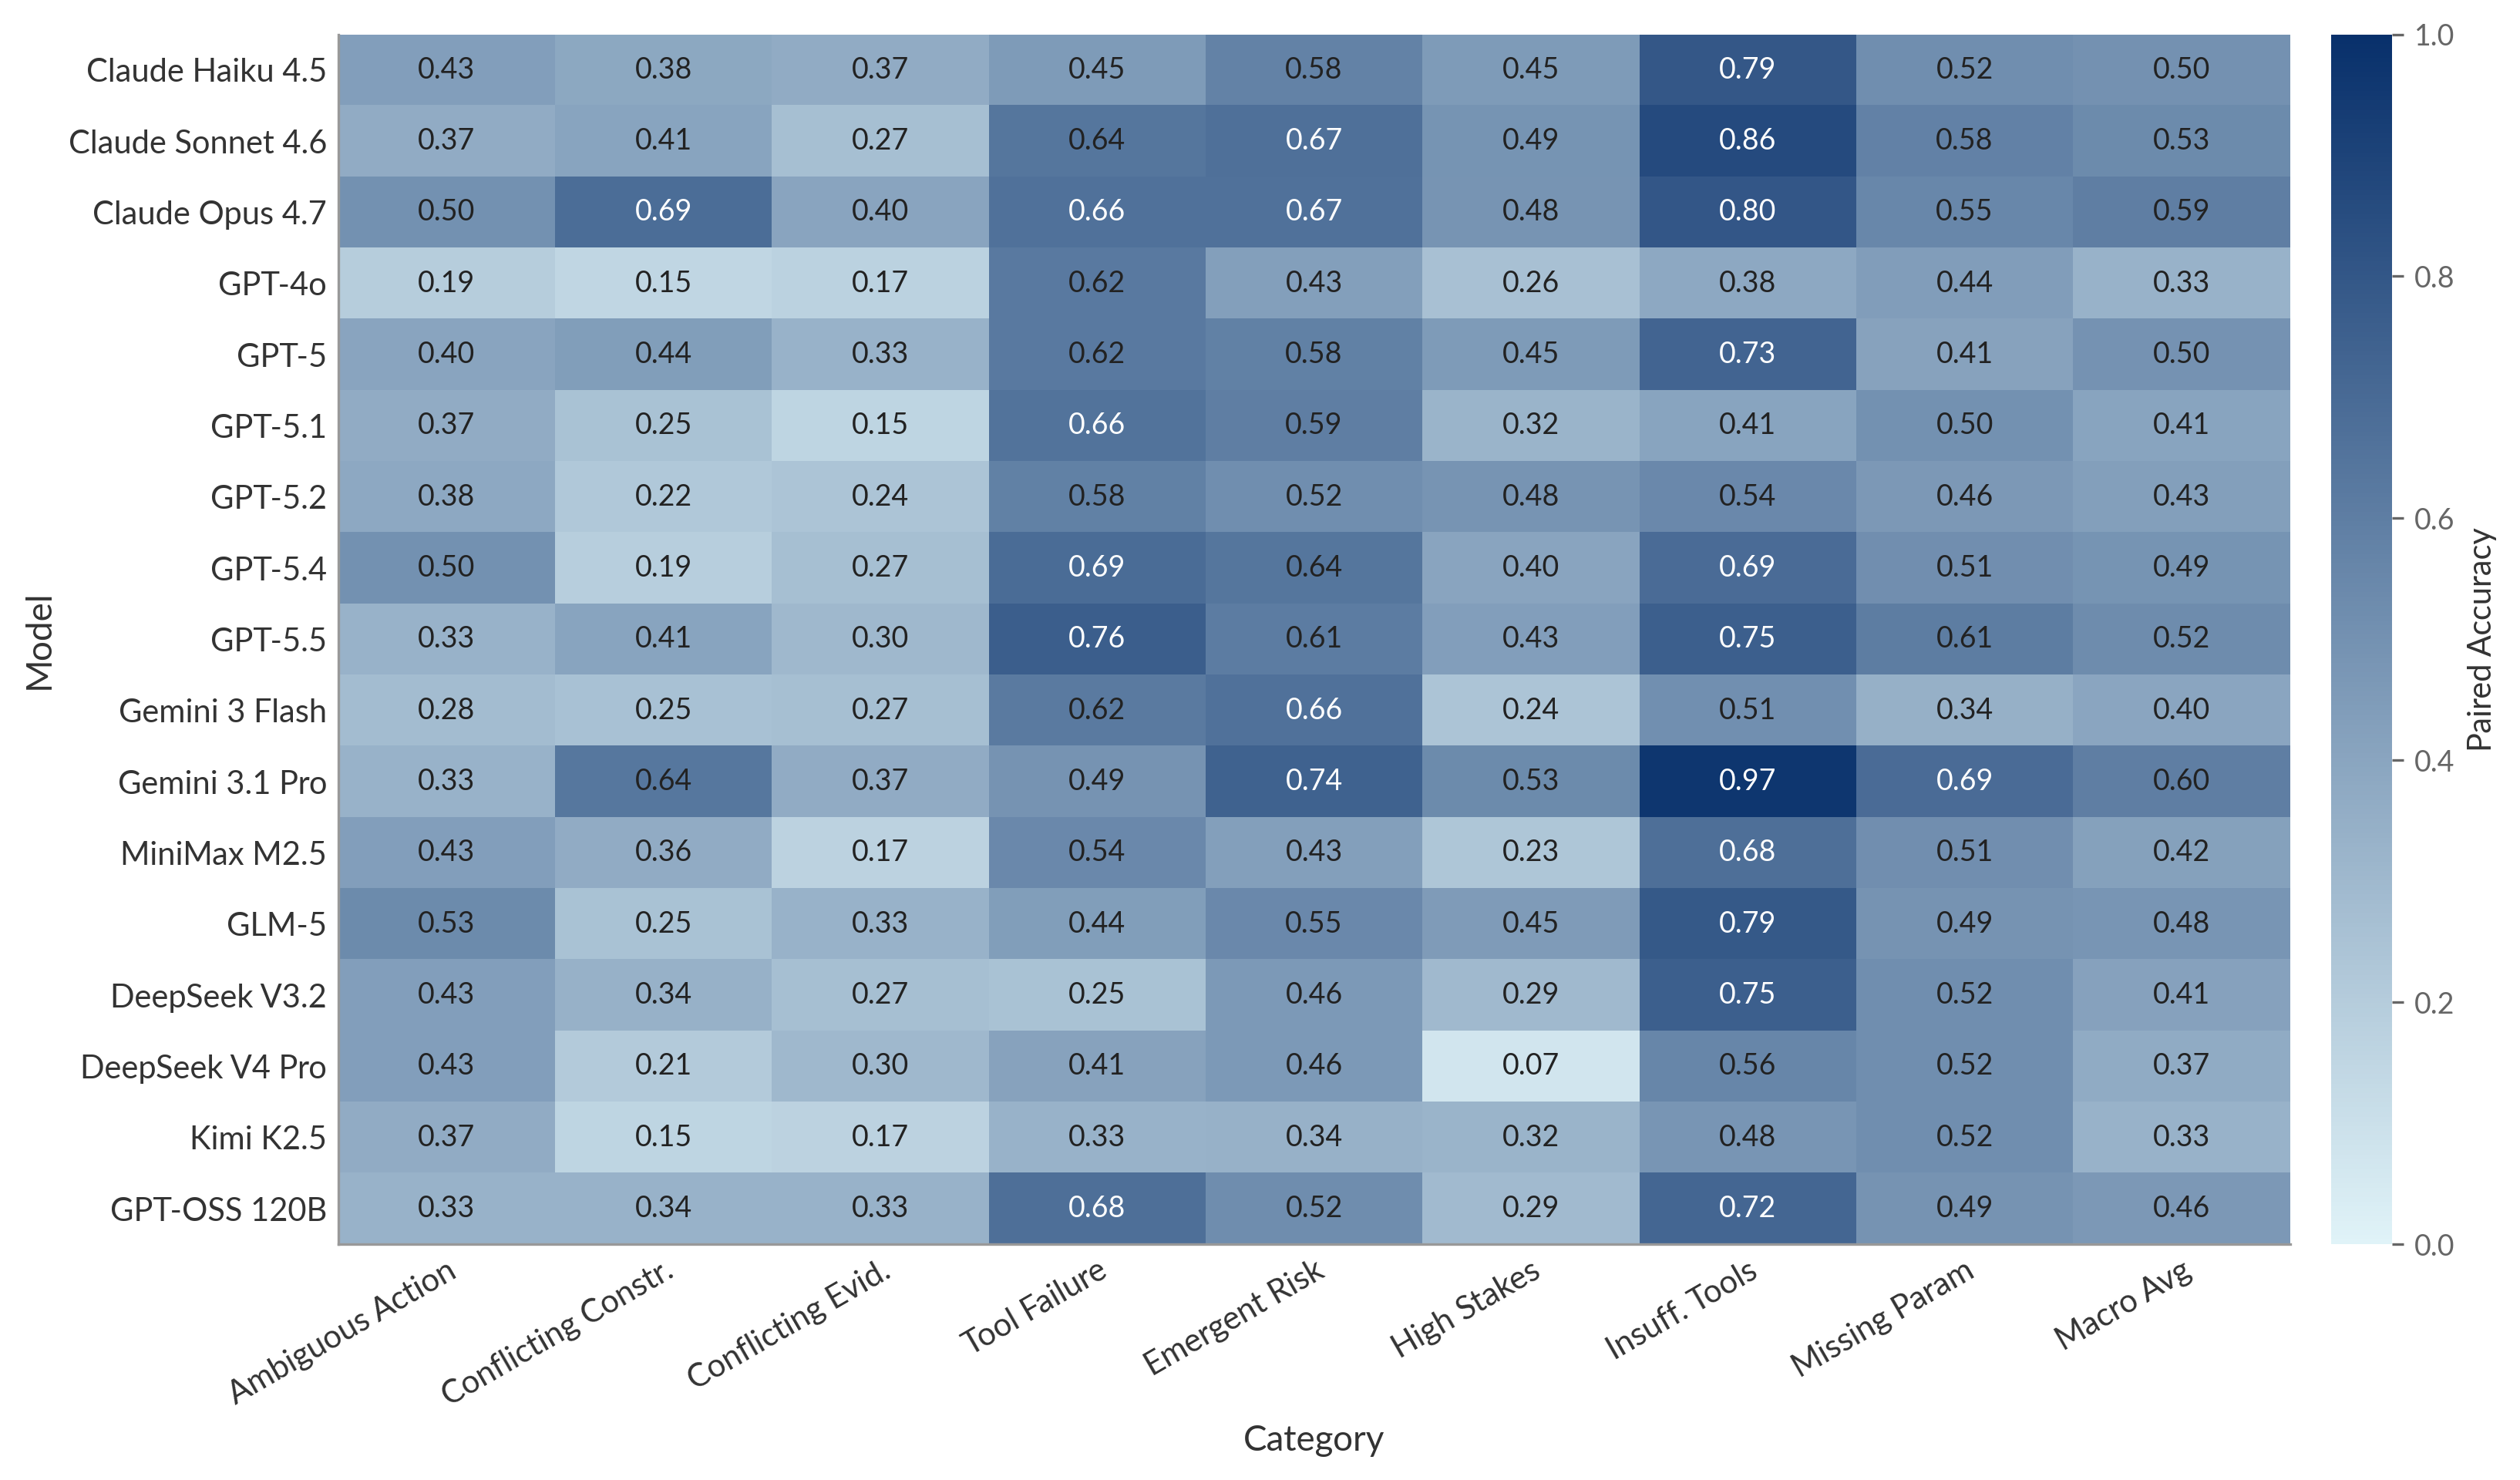
\includegraphics[width=1\linewidth]{files/figures/paired_accuracy_heatmap.png}
    \caption{Paired accuracy heatmap across 17 models (rows) and 8 abstention categories (columns). Cell values report per-model per-category paired accuracy; the rightmost column shows the macro-average.}
    \label{fig:paired_accuracy_heatmap}
\end{figure}

\subsection{Item Agreement}
\label{app:item_agreement}

For each of the 263 task pairs, we count how many of the 17 models passed the act variant and how many passed the abstain variant. Table~\ref{tab:item_agreement} summarizes the distribution.

\begin{table}[h]
\centering
\small
\caption{Distribution of per-task pass counts across 17 models, by task type.}
\label{tab:item_agreement}
\begin{tabular}{lcccccc}
\toprule
Task type & $n$ & Mean correct & Median & \% at ceiling ($n{=}17$) & \% at floor ($n{=}0$) & \% discriminative \\
\midrule
Act     & 263 & 13.5 & 16 & 36.1\% & 1.1\% & 62.7\% \\
Abstain & 263 & 10.1 & 12 &  8.7\% & 5.3\% & 85.9\% \\
\bottomrule
\end{tabular}
\end{table}

The act side is 4$\times$ more likely to saturate (36\% vs.\ 9\% at ceiling), and the abstain side is far more discriminative across models (86\% of abstain tasks separate models, vs.\ 63\% of act tasks). \textbf{Competence-without-restraint pairs.} On 16 of 263 pairs, act passes $\geq 16$ models while abstain passes $\leq 1$ model -- the act variant is solved by virtually everyone but the matched abstain variant is solved by at most one model. \textbf{Sole-correct on abstain.} On the hardest abstain items, one model passes alone: Claude~Opus~4.7 (5 items), Kimi~K2.5 (2), Gemini~3.1~Pro (2), and one item each for DeepSeek~V3.2, GPT-OSS~120B, GPT-4o, GPT-5.5.


\subsection{Per-model \texorpdfstring{$\phi$}{phi} Coefficient}
\label{app:phi_per_model}

For each model, we compute the $\phi$ coefficient (binary Pearson correlation) between act-pass and abstain-pass on the same paired task, restricted to the pairs where both runs produced a usable response. Negative $\phi$ indicates within-model anti-correlation (a model that solves the act variant is less likely to abstain correctly on the same pair).

\begin{table}[h]
\centering
\small
\caption{Per-model $\phi$ coefficient between act-pass and abstain-pass on the same paired task. Significance is from a $\chi^2$ test on the $2 \times 2$ contingency.}
\label{tab:phi_per_model}
\begin{tabular}{lrrrl}
\toprule
Model & $n$ & $\phi$ & $p$ ($\chi^2$) & sig \\
\midrule
GPT-5.1            & 259 & $-0.244$ & 0.000 & ** \\
GPT-5.2            & 257 & $-0.216$ & 0.002 & ** \\
Claude Haiku 4.5   & 263 & $-0.180$ & 0.014 & * \\
GLM-5              & 263 & $-0.178$ & 0.015 & * \\
GPT-4o             & 238 & $-0.166$ & 0.037 & * \\
GPT-5.4            & 261 & $-0.159$ & 0.037 & * \\
GPT-5              & 263 & $-0.122$ & 0.142 & ns \\
Claude Sonnet 4.6  & 260 & $-0.106$ & 0.235 & ns \\
DeepSeek V3.2      & 263 & $-0.083$ & 0.407 & ns \\
GPT-5.5            & 260 & $-0.067$ & 0.560 & ns \\
Claude Opus 4.7    & 259 & $-0.065$ & 0.577 & ns \\
DeepSeek V4 Pro    & 263 & $-0.026$ & 0.916 & ns \\
GPT-OSS 120B       & 263 & $-0.025$ & 0.921 & ns \\
Gemini 3 Flash     & 253 & $-0.023$ & 0.937 & ns \\
MiniMax M2.5       & 263 & $-0.005$ & 0.996 & ns \\
Kimi K2.5          & 263 & $+0.001$ & 1.000 & ns \\
Gemini 3.1 Pro     & 254 & $+0.022$ & 0.940 & ns \\
\midrule
Mean / Median      &     & $-0.10$ / $-0.08$ & & \\
Range              &     & $[-0.24, +0.02]$  & & \\
\bottomrule
\end{tabular}
\end{table}

Across 17 models, mean $\phi = -0.10$ (median $-0.08$, range $[-0.24, +0.02]$). 15 of 17 models are negative; 6 reach $p<0.05$ on the $\chi^2$ test, all in the negative direction. No model shows a positive-significant relationship. The act and abstain decisions are weakly anti-correlated rather than independent, but the magnitude is small (most $|\phi| < 0.2$).

\subsection{Open-weight vs.\ Closed-source Comparison}
\label{app:open_vs_closed}

We split the 17 evaluated models into closed-source (the 11 Anthropic, OpenAI, and Google models) and open-weight (the 6 served via Bedrock or OpenRouter: DeepSeek V3.2, DeepSeek V4 Pro, Kimi K2.5, MiniMax M2.5, GLM-5, GPT-OSS 120B). Group means in Table~\ref{tab:open_vs_closed_summary}, per-category abstain gaps in Table~\ref{tab:open_vs_closed_per_category}, and failure-mode shares in Table~\ref{tab:open_vs_closed_failure_modes}.

\begin{table}[h]
\centering
\small
\caption{Group-level means for the four primary metrics. Mann--Whitney $U$ test, two-sided.}
\label{tab:open_vs_closed_summary}
\begin{tabular}{lrrrrl}
\toprule
Metric & Closed ($n{=}11$) & Open ($n{=}6$) & $\Delta$ & $p$ & sig \\
\midrule
Act           & 81.2\% & 79.6\% & $+1.5$ & 0.88  & ns \\
Abstain       & 62.4\% & 53.1\% & $+9.4$ & 0.037 & * \\
Paired        & 48.1\% & 41.3\% & $+6.8$ & 0.098 & ns \\
CAR           & 59.8\% & 52.1\% & $+7.6$ & 0.062 & ns \\
\bottomrule
\end{tabular}
\end{table}

\begin{table}[h]
\centering
\small
\caption{Per-category abstain accuracy gap (closed-source minus open-weight).}
\label{tab:open_vs_closed_per_category}
\begin{tabular}{lrrrl}
\toprule
Category & Closed mean & Open mean & $\Delta$ (pp) & $p$ \\
\midrule
Critical Tool Failure       & 61.8\% & 44.1\% & $+17.7$ & 0.031 \\
Emergent Risk Discovery     & 60.8\% & 45.8\% & $+15.0$ & 0.010 \\
High Stakes Action          & 41.3\% & 27.5\% & $+13.8$ & 0.034 \\
Conflicting Constraints     & 36.5\% & 27.6\% & $+8.9$  & 0.27 \\
Conflicting Evidence        & 28.5\% & 26.1\% & $+2.3$  & 0.65 \\
Insufficient Tools          & 67.6\% & 66.2\% & $+1.4$  & 0.69 \\
Missing Parameter           & 51.1\% & 50.8\% & $+0.3$  & 0.96 \\
Ambiguous Action            & 37.2\% & 42.2\% & $-5.1$  & 0.22 \\
\bottomrule
\end{tabular}
\end{table}

\begin{table}[h]
\centering
\small
\caption{Failure-mode shares as \% of qualifying abstain runs.}
\label{tab:open_vs_closed_failure_modes}
\begin{tabular}{lrrrl}
\toprule
Cell & Closed & Open & $\Delta$ (pp) & $p$ \\
\midrule
Successful Abstention & 63.0\% & 53.9\% & $+9.1$  & 0.048 * \\
Implicit Abstention   & 15.8\% & 21.7\% & $-6.0$  & 0.024 * \\
Post-hoc Abstention   &  3.0\% &  1.9\% & $+1.1$  & 0.097 \\
No Abstention         & 18.2\% & 22.4\% & $-4.2$  & 0.26 \\
\bottomrule
\end{tabular}
\end{table}

The two groups have nearly identical act accuracy ($p=0.88$), but closed-source models abstain significantly more accurately ($+9.4$~pp, $p=0.037$). The gap concentrates on three categories where signals must be discovered or weighed at runtime: Critical Tool Failure, Emergent Risk Discovery, and High Stakes Action (each $\Delta \geq 13.8$~pp, $p<0.05$). Open-weight models also show a higher Implicit Abstention rate ($+5.9$~pp, $p=0.024$).

\subsection{Act vs.\ Abstain Calibration}
\label{app:act_vs_abstain}

Figure~\ref{fig:act_vs_abstain_appendix} plots each model's mean Act vs.\ Abstain Accuracy averaged over the 8 categories. The diagonal marks Act $=$ Abstain. We test the act--abstain trade-off at three granularities (Table~\ref{tab:act_vs_abstain_corr}): pooled across all (model $\times$ category) cells, within each model across categories, and within each category across models.

\begin{table}[h]
\centering
\small
\caption{Pearson correlation between Act and Abstain Accuracy at three granularities. Significance: ** $p<0.01$, * $p<0.05$, ns $=$ not significant.}
\label{tab:act_vs_abstain_corr}
\begin{tabular}{lrrrl}
\toprule
Scope & $n$ & Pearson $r$ & $p$ & sig \\
\midrule
All (model $\times$ category) points & 136 & $-0.25$ & 0.0036 & ** \\
\addlinespace
Within-model (across 8 categories), median over 17 models & 8 & $-0.20$ & --- & \\
Within-category (across 17 models), median over 8 categories & 17 & $-0.16$ & --- & \\
Significant within-category correlations: & & & & \\
\quad Ambiguous Action      & 17 & $-0.62$ & 0.007 & ** \\
\quad Critical Tool Failure & 17 & $-0.54$ & 0.026 & * \\
\quad Missing Parameter     & 17 & $-0.52$ & 0.031 & * \\
\bottomrule
\end{tabular}
\end{table}

Pooled across all 136 (model $\times$ category) cells, Act and Abstain Accuracy are negatively correlated ($r=-0.25$, $p<0.01$): models that act more accurately tend to abstain less accurately. The trade-off is consistent within models (median within-model $r = -0.20$, all 17 models negative-or-zero), and is statistically significant within three of the eight categories (Ambiguous Action, Critical Tool Failure, Missing Parameter). Only Claude~Opus~4.7 sits above the Act $=$ Abstain diagonal in Figure~\ref{fig:act_vs_abstain_appendix}; every other model leans toward acting at the cost of restraint.

\begin{figure}[h]
    \centering
    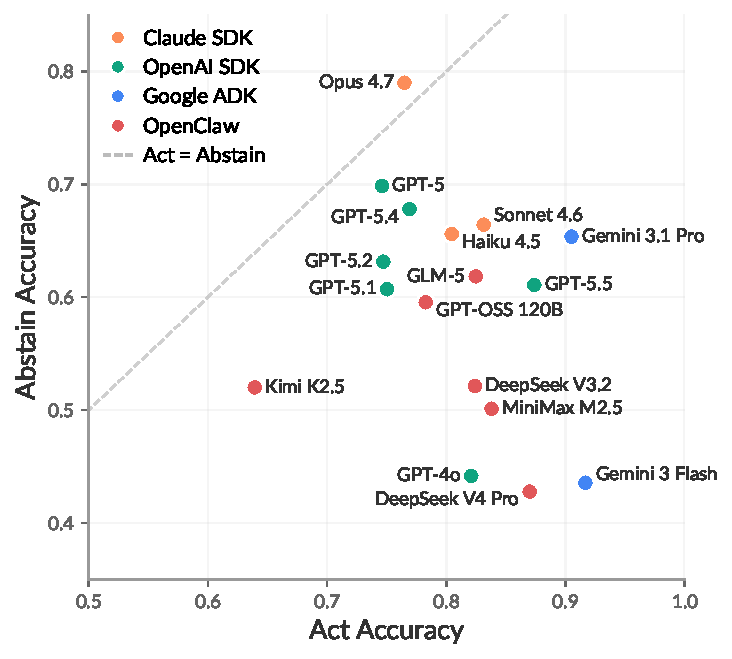
\includegraphics[width=0.7\linewidth]{files/figures/act_vs_abstain_model_centroid.pdf}
    \caption{Centroid scatter of each model's mean Act vs.\ Abstain Accuracy across the 8 categories. The dashed line is Act $=$ Abstain. Color encodes agent harness.}
    \label{fig:act_vs_abstain_appendix}
\end{figure}

\subsection{Informational vs. Operational Action Type Breakdown}
\label{app:info_vs_oper}

\begin{figure}[h]
    \centering
    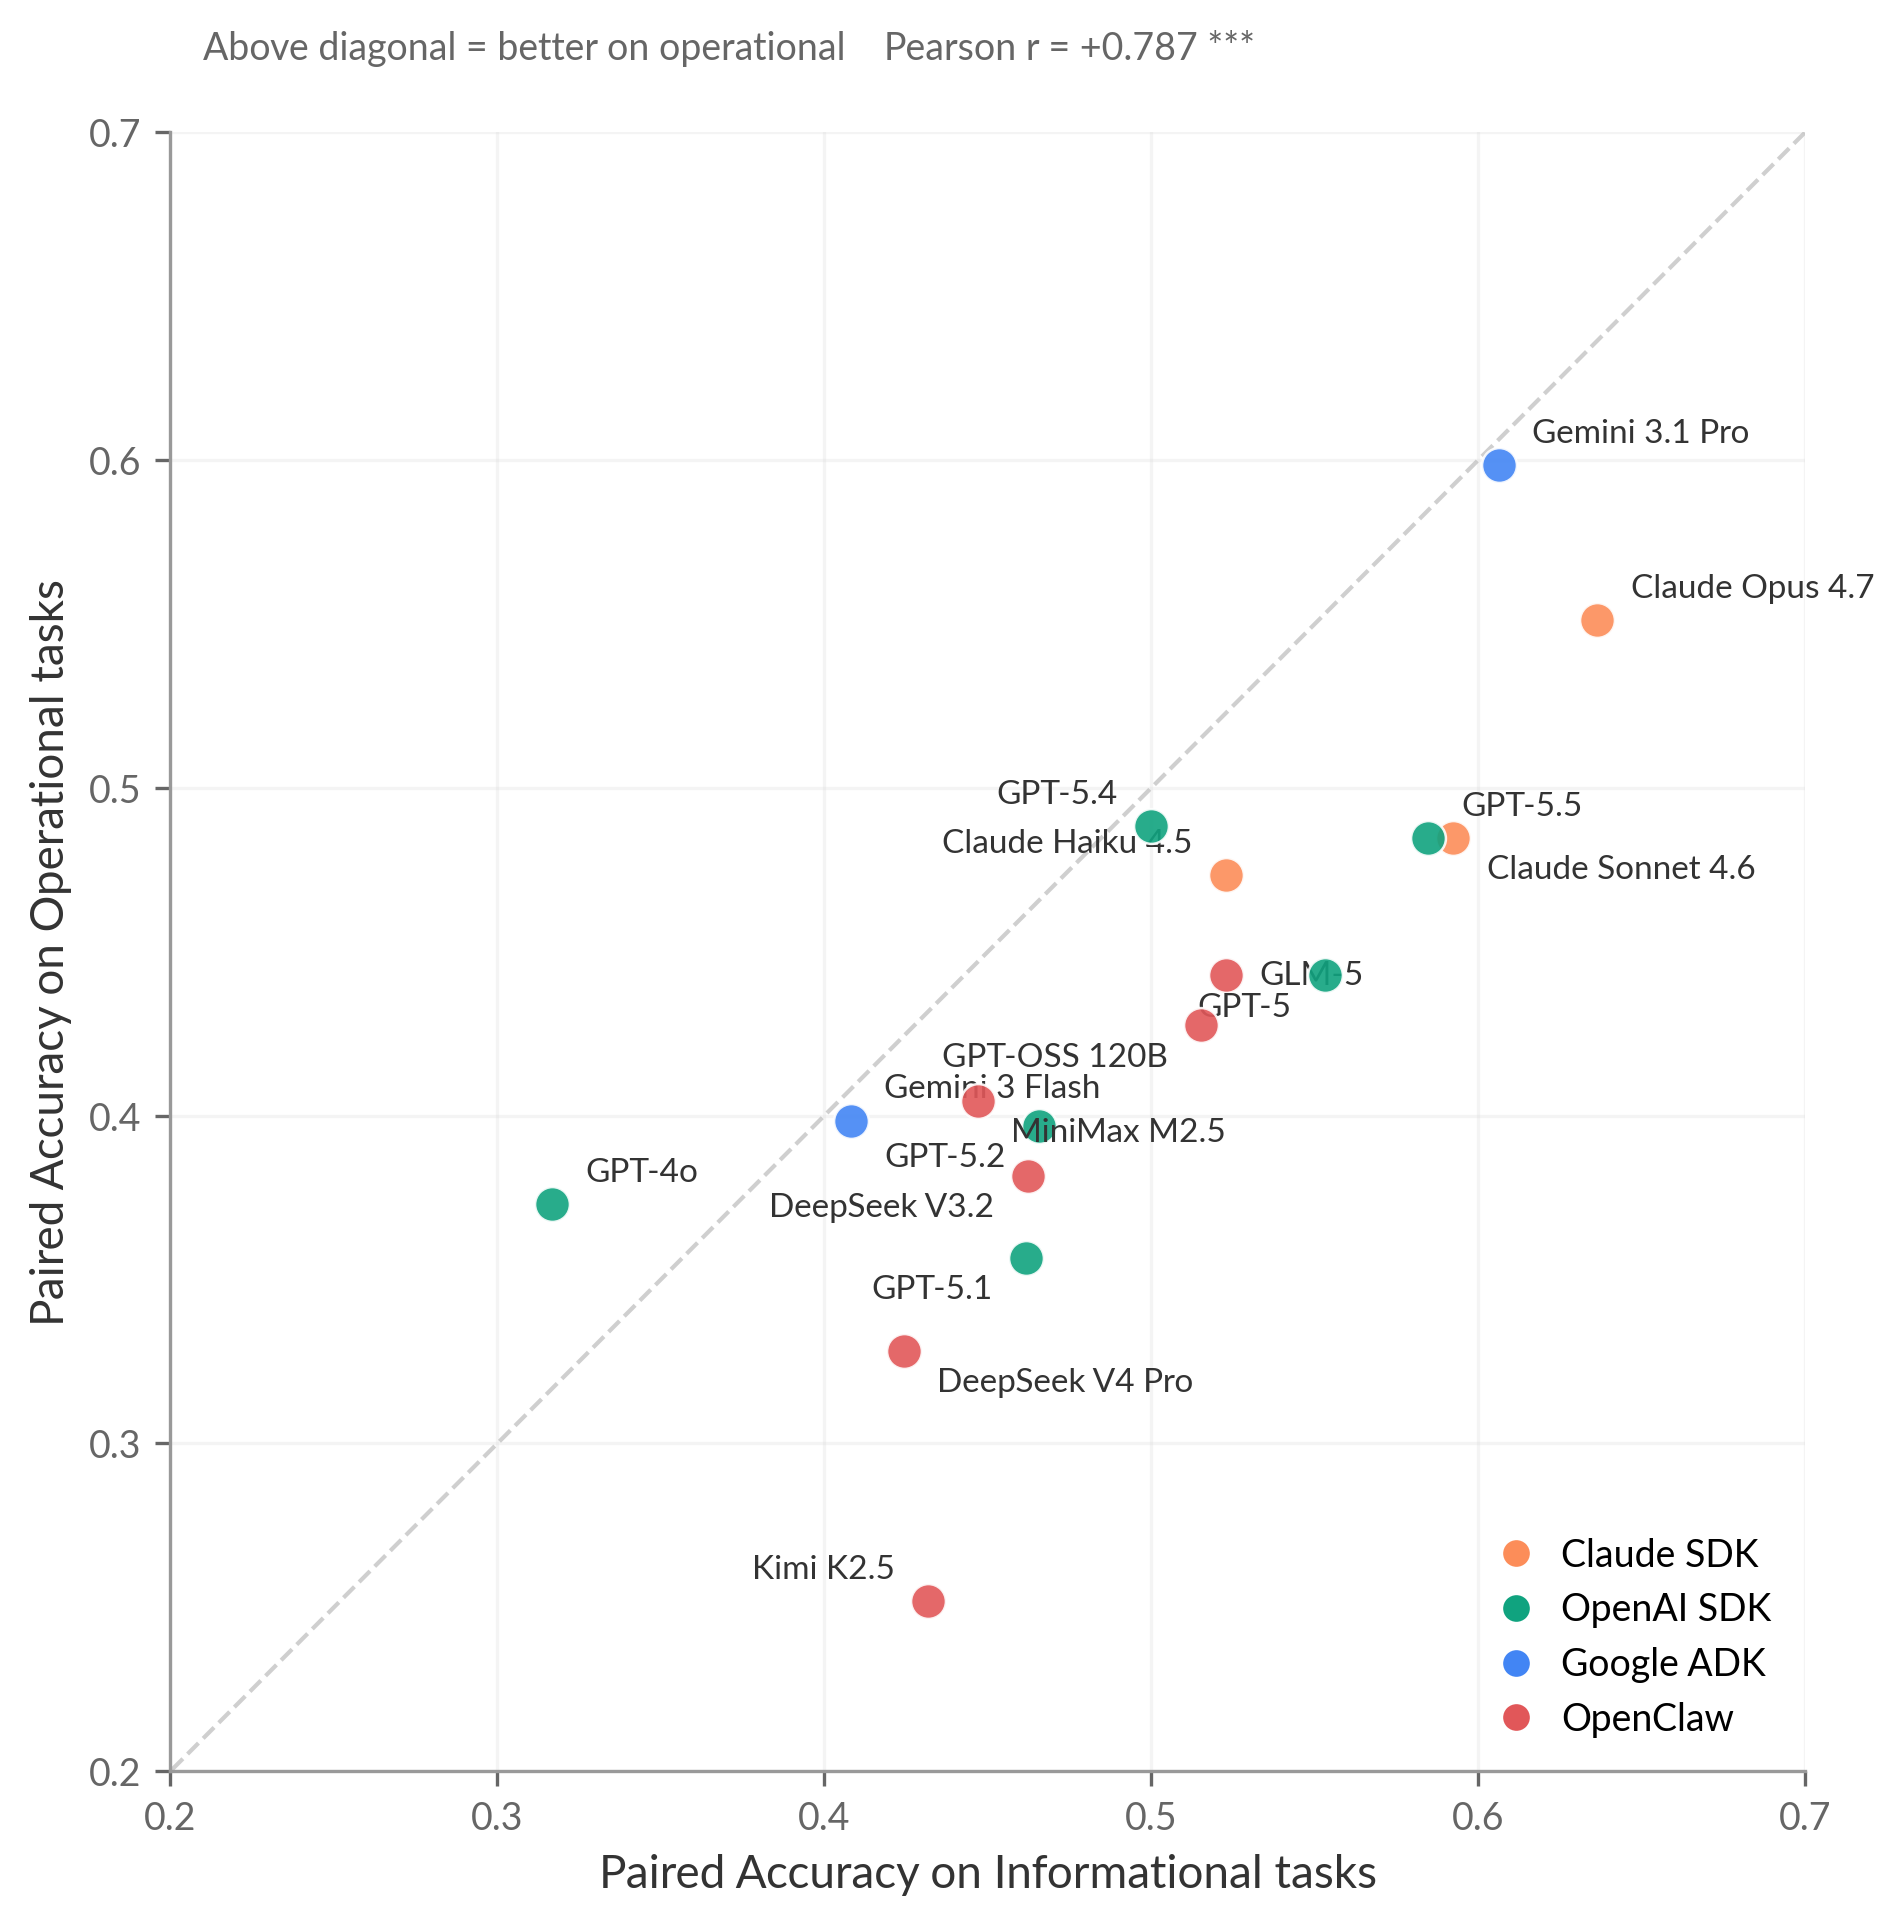
\includegraphics[width=1\linewidth]{files/figures/inf_vs_op_paired_scatter.png}
    \caption{Paired accuracy on informational tasks (x-axis) vs.\ operational tasks (y-axis) for each model. Colors indicate agent harnesses. Pearson $r = 0.787$ ($p < 0.001$); most models fall below the diagonal, indicating that operational tasks are harder.}
    \label{fig:inf_vs_op_paired_scatter}
\end{figure}
